\documentclass[journal,12pt,twocolumn]{IEEEtran}

\usepackage{setspace}
\usepackage{gensymb}
\singlespacing
\usepackage[cmex10]{amsmath}

\usepackage{amsthm}

\usepackage{mathrsfs}
\usepackage{txfonts}
\usepackage{stfloats}
\usepackage{bm}
\usepackage{cite}
\usepackage{cases}
\usepackage{subfig}

\usepackage{longtable}
\usepackage{multirow}

\usepackage{enumitem}
\usepackage{mathtools}
\usepackage{steinmetz}
\usepackage{tikz}
\usepackage{circuitikz}
\usepackage{verbatim}
\usepackage{tfrupee}
\usepackage[breaklinks=true]{hyperref}
\usepackage{graphicx}
\usepackage{tkz-euclide}

\usetikzlibrary{calc,math}
\usepackage{listings}
    \usepackage{color}                                            %%
    \usepackage{array}                                            %%
    \usepackage{longtable}                                        %%
    \usepackage{calc}                                             %%
    \usepackage{multirow}                                         %%
    \usepackage{hhline}                                           %%
    \usepackage{ifthen}                                           %%
    \usepackage{lscape}     
\usepackage{multicol}
\usepackage{chngcntr}

\DeclareMathOperator*{\Res}{Res}

\renewcommand\thesection{\arabic{section}}
\renewcommand\thesubsection{\thesection.\arabic{subsection}}
\renewcommand\thesubsubsection{\thesubsection.\arabic{subsubsection}}

\renewcommand\thesectiondis{\arabic{section}}
\renewcommand\thesubsectiondis{\thesectiondis.\arabic{subsection}}
\renewcommand\thesubsubsectiondis{\thesubsectiondis.\arabic{sub subsection}}


\hyphenation{optical networks semiconduc-tor}
\def\inputGnumericTable{}                                 %%

\lstset{
%language=C,
frame=single, 
breaklines=true,
columns=fullflexible
}
\date{March 2021}

\begin{document}

\newcommand{\BEQA}{\begin{eqnarray}}
\newcommand{\EEQA}{\end{eqnarray}}
\newcommand{\define}{\stackrel{\triangle}{=}}
\bibliographystyle{IEEEtran}
\raggedbottom
\setlength{\parindent}{0pt}
\providecommand{\mbf}{\mathbf}
\providecommand{\pr}[1]{\ensuremath{\Pr\left(#1\right)}}
\providecommand{\qfunc}[1]{\ensuremath{Q\left(#1\right)}}
\providecommand{\fn}[1]{\ensuremath{f\left(#1\right)}}
\providecommand{\e}[1]{\ensuremath{E\left(#1\right)}}
\providecommand{\sbrak}[1]{\ensuremath{{}\left[#1\right]}}
\providecommand{\lsbrak}[1]{\ensuremath{{}\left[#1\right.}}
\providecommand{\rsbrak}[1]{\ensuremath{{}\left.#1\right]}}
\providecommand{\brak}[1]{\ensuremath{\left(#1\right)}}
\providecommand{\lbrak}[1]{\ensuremath{\left(#1\right.}}
\providecommand{\rbrak}[1]{\ensuremath{\left.#1\right)}}
\providecommand{\cbrak}[1]{\ensuremath{\left\{#1\right\}}}
\providecommand{\lcbrak}[1]{\ensuremath{\left\{#1\right.}}
\providecommand{\rcbrak}[1]{\ensuremath{\left.#1\right\}}}
\theoremstyle{remark}
\newtheorem{rem}{Remark}
\newcommand{\sgn}{\mathop{\mathrm{sgn}}}
\providecommand{\abs}[1]{\vert#1\vert}
\providecommand{\res}[1]{\Res\displaylimits_{#1}} 
\providecommand{\norm}[1]{\lVert#1\rVert}
%\providecommand{\norm}[1]{\lVert#1\rVert}
\providecommand{\mtx}[1]{\mathbf{#1}}
\providecommand{\mean}[1]{E[ #1 ]}
\providecommand{\fourier}{\overset{\mathcal{F}}{ \rightleftharpoons}}
%\providecommand{\hilbert}{\overset{\mathcal{H}}{ \rightleftharpoons}}
\providecommand{\system}{\overset{\mathcal{H}}{ \longleftrightarrow}}
	%\newcommand{\solution}[2]{\textbf{Solution:}{#1}}
\newcommand{\solution}{\noindent \textbf{Solution: }}
\newcommand{\cosec}{\,\text{cosec}\,}
\providecommand{\dec}[2]{\ensuremath{\overset{#1}{\underset{#2}{\gtrless}}}}
\newcommand{\myvec}[1]{\ensuremath{\begin{pmatrix}#1\end{pmatrix}}}
\newcommand{\mydet}[1]{\ensuremath{\begin{vmatrix}#1\end{vmatrix}}}
\numberwithin{equation}{subsection}
\makeatletter
\vspace{3cm}
\title{ASSIGNMENT 3}
\author{MANIKANTA VALLEPU - AI20BTECH11014}
\maketitle
\newpage
\bigskip
\renewcommand{\thetable}{\theenumi}
Download all python codes from 
\begin{lstlisting}
https://github.com/manik2255/AI1103-PROBABILITY-AND-RANDOM-VARIABLES/blob/main/ASSIGNMENT_3/assign_3.py
\end{lstlisting}
%
and latex-tikz codes from 
%
\begin{lstlisting}
https://github.com/manik2255/AI1103-PROBABILITY-AND-RANDOM-VARIABLES/blob/main/ASSIGNMENT_3/ASSIGNMENT_3.tex
\end{lstlisting}
\section{GATE 2017 MA PROBLEM.47 }
Let X and Y be independent and identically distributed random variables with probability mass function $p(n) = 2^{-n}$,$n=1,2,\dots$\\
Then $pr(X\ge 2Y)$ equals 

\section{Solution}
given,\\
\begin{align}
pr(X=x) =2^{-x} ,x=1,2,\dots \label{a}\\
pr(Y=y) =2^{-y} ,y=1,2,\dots \label{b}
\end{align}
We need to find $pr(X\ge 2Y)$,which is also can be written as
\begin{align}
    pr(X\ge 2Y) &=\sum_{y=1}^{\infty}pr(X \ge 2y|Y=y)
\end{align}
as,X and Y are independent random variables
\begin{align}
    pr(X\ge 2Y) &=\sum_{y=1}^{\infty}pr(X \ge 2y)pr(Y=y)\\
               &=\sum_{y=1}^{\infty}(1-pr(X < 2y))pr(Y=y) \label{c}
\end{align}
using \eqref{a} and \eqref{b} in \eqref{c},
\begin{align}
               &=\sum_{y=1}^{\infty}(1- \sum_{i=1}^{2y-1}2^{-i})(2^{-y})\\
               &=\sum_{y=1}^{\infty}(1-(1-2^{-(2y-1)}))(2^{-y})\\
               &=\sum_{y=1}^{\infty}2^{-(3y-1)}\\
               &=\frac{2}{7}
\end{align}
\begin{figure}[ht]
    \centering
    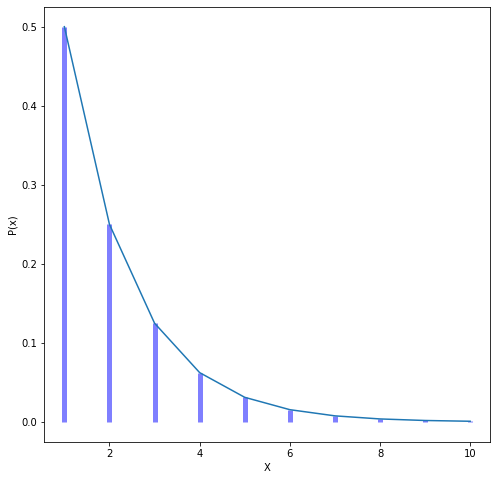
\includegraphics[width=\columnwidth]{Fig_1.png}
    \caption{Pmf of random variable X}
    \label{Fig_1}
\end{figure}
\begin{figure}[ht]
    \centering
    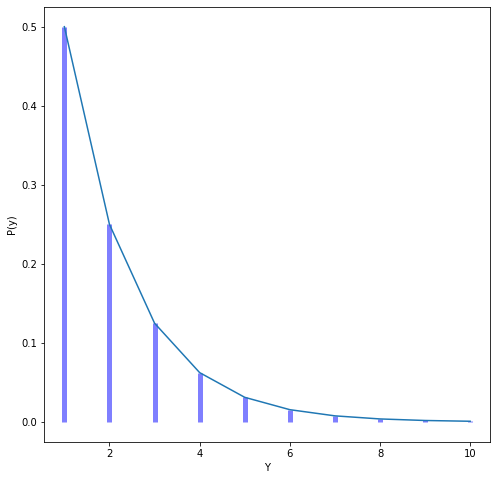
\includegraphics[width=\columnwidth]{Fig_2.png}
    \caption{Pmf of random variable Y}
    \label{Fig_2}
\end{figure}
Finding the probability using cumulative distribution,
Let $F_X(x)$ be the cumulative distribution function of random variable X.
\begin{align}
    F_X(x)&=\pr{X<x}
\end{align}\label{d}
As it is a discrete probability distribution, $F_X(x)$ can be written as,
\begin{align}
    F_X(x)&= \sum_{i=1}^{x-1}\pr{X=x} 
\end{align}\label{t}
using \eqref{a} in \eqref{t}
\begin{align}
    F_X(x)&=\sum_{i=1}^{x-1}2^{-i}\\
         &=1-2^{-(x-1)} 
\end{align}
Cumulative distribution function (CDF) of random variable X is given by,
\begin{align}
    F_X(x)&=1-2^{-(x-1)} ,x=1,2,\dots
\end{align} \label{3}
We need to find $pr(X\ge 2Y)$,which is also can be written as
\begin{align}
    pr(X\ge 2Y) &=\sum_{y=1}^{\infty}pr(X \ge 2y|Y=y)
\end{align}
As,X and Y are independent random variables
\begin{align}
    pr(X\ge 2Y) &=\sum_{y=1}^{\infty}pr(X \ge 2y)pr(Y=y)\\
               &=\sum_{y=1}^{\infty}(1-pr(X < 2y))pr(Y=y) \label{4}
\end{align}
using \eqref{b} and \eqref{3} in \eqref{4},
\begin{align}
pr(X\ge 2Y) &=\sum_{y=1}^{\infty}(1-(1-2^{-(2y-1)}))(2^{-y})\\
           &=\sum_{y=1}^{\infty}2^{-(3y-1)}\\
               &=\frac{2}{7}
\end{align}
\begin{figure}[ht]
    \centering
    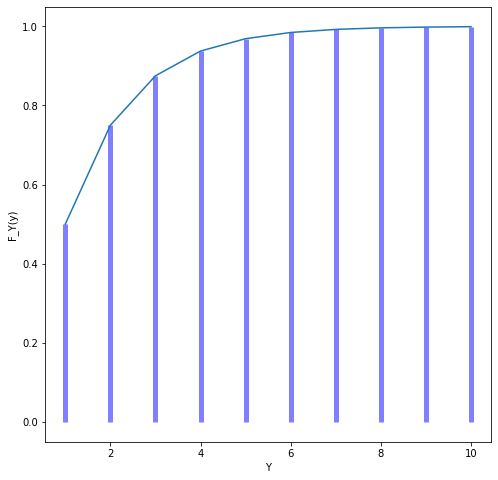
\includegraphics[width=\columnwidth]{Fig_3.png}
    \caption{cdf of random variable Y}
    \label{Fig_3}
\end{figure}
\end{document}
